 \documentclass[11pt]{article}
 \usepackage{amsmath, alltt, amssymb, xspace, times, epsfig,
   algpseudocode, color, multirow, listings, mathtools}

\usepackage[font=small,labelfont=bf,textfont=it]{caption}
\usepackage{subcaption}
\DeclarePairedDelimiter{\ceil}{\lceil}{\rceil}
\DeclarePairedDelimiter{\floor}{\lfloor}{\rfloor}

 \setlength{\evensidemargin}{0in} \setlength{\oddsidemargin}{0in}
 \setlength{\textwidth}{6.5in} \setlength{\textheight}{8.5in}
 \setlength{\topmargin}{0in} \setlength{\headheight}{0in}


\begin{document}
 \thispagestyle{empty}

 \noindent \textbf{CS525: Parallel Computing\hspace*{\fill}Spring 2013} 
 \begin{center}
   {\LARGE Homework \#4\\\small Josh Reese}\\
 \end{center}
 {\bf Problem 1} Values for $t_s$ and $t_w$ were obtained on the mc
 cluster by sending point to point messages of increasing size between
 two machines. Each
 message was sent 50 times and the average return trip was used for
 computation. To compute $t_s$ I used the value obtained for the
 smaller message (1, 10, and 50 bytes). This value turned out to be
 approximately $60\mu s$. From this $t_w$ was obtained by examining
 the times for larger messages (10MB, 20MB) and computed by
 $(T-t_s)/m$. Where $T$ was the average roundtrip time. This value
 turned out to be approximately $0.0085\mu s$.\\

 {\bf Problem 2} To test these operations a similar strategy to that
 of problem 1 was instituted. The main difference here was that I also
 varied the number of nodes involved in the communication. This range
 was [2,4,8,12,16]. However, results for 2 and 4 weren't revealing so
 only 8, 12, and 16 are reported in the graphs. Each graph is broken
 up by number of processors on the x-axis and inside each group of
 processors the times for increasing message sizes is reported. These
 are the values obtained empirically using MPI and theoretically using
 the equations found in the text.\\
 \begin{figure}[h]
   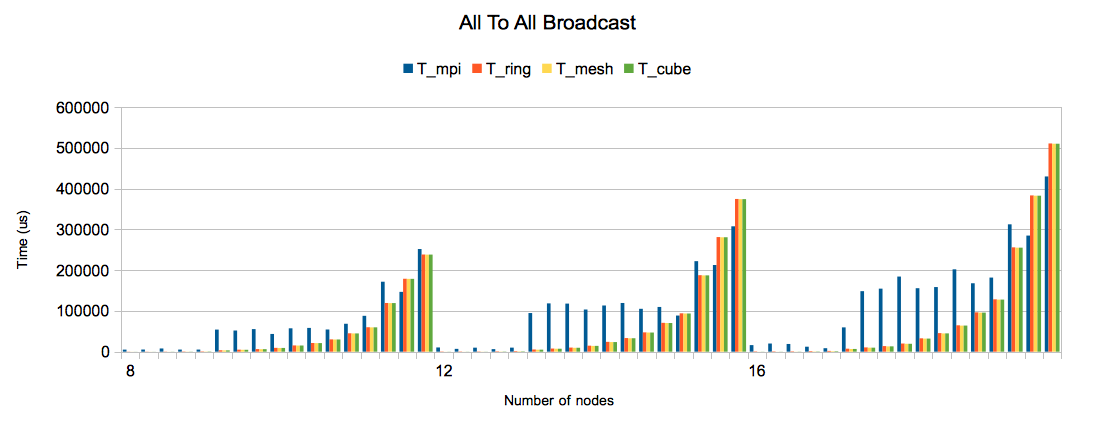
\includegraphics[width=\textwidth]{images/all2all.png}
   \caption{All to all broadcast times for Problem 2}
 \end{figure}
 \begin{figure}[h!]
   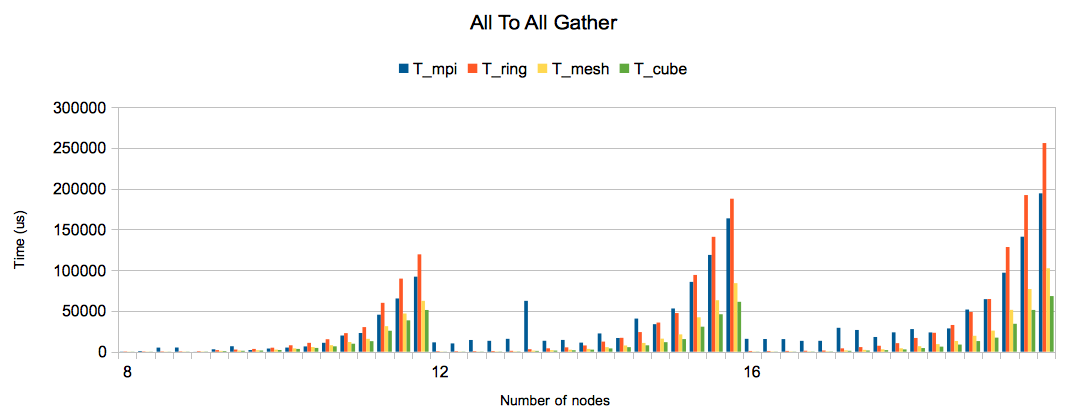
\includegraphics[width=\textwidth]{images/allgather.png}
   \caption{All to all gather times for Problem 2}
 \end{figure}
 \begin{figure}[ht]
   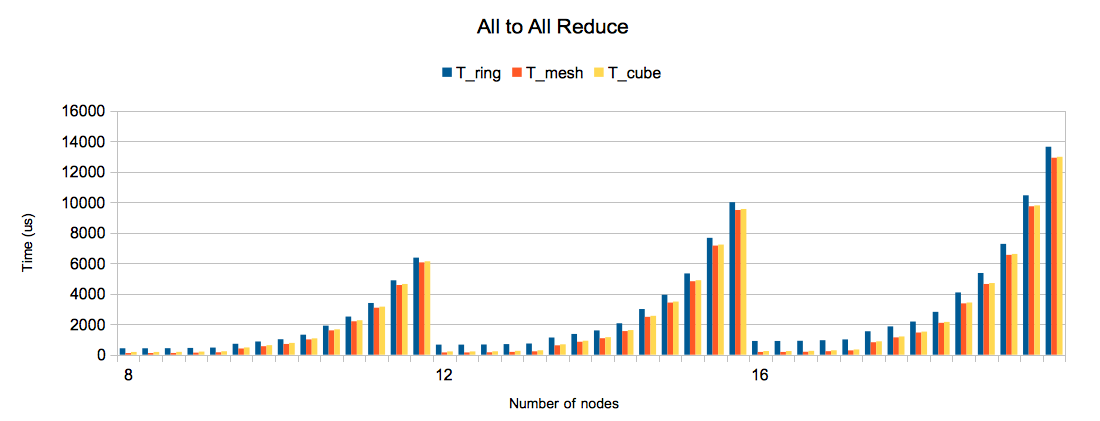
\includegraphics[width=\textwidth]{images/allreduce.png}
   \caption{All to all reduce times for Problem 2}
 \end{figure}

 {\bf 5.1 (Amdahl's law [Amd67])} If a problem of size $W$ has a serial
 component $W_s$, prove that $W/W_s$ is an upper bound on its speedup, no
 matter how many processing elements are used.\\\\
 We define speedup as $S = \frac{T_s}{T_p}$, the sequential time
 as $T_s = W$ and the parallel time as $T_p = W_s +
 \frac{W+T_o(W,p)}{p}$. This last term, the parallel time, is
 taken from the parallel time discussed in the text and adding a
 $W_s$ component to is. The reason for this is that $W_s$ is a
 serial component and the time must be added to the parallel
 run time. This time is not related to the number of processors
 used because it must always be executed in serial. With these
 definitions we can formulate an equation for the speedup as:
 $$ \begin{array}{lcc}
   S & = & \frac{T_s}{T_p}\\
   & = & \frac{W}{W_s + \frac{W+T_o(W,p)}{p}}
 \end{array} $$
 From this we can see that even if $p$ grows to infinity and the
 second term vanishes from the denominator we are still left with
 $\frac{W}{W_s}$ as the speedup. Thus giving us an upper bound.\\
 
 {\bf 5.2 (Superlinear speedup)} Consider the search tree shown in
 Figure 5.10(a), in which the dark node represents the solution.\\
 a. If a sequential search of the tree is performed using the
 standard depth-first search (DFS) algorithm (Section 11.2.1), how
 much time does it take to find the solution if traversing each
 arc of the tree takes one unit of time?\\\\
 b. Assume that the tree is partitioned between two processing
 elements that are assigned to do the search job, as shown in
 Figure 5.10(b). If both processing elements perform a DFS on
 their respective halves of the tree, how much time does it take
 for the solution to be found? What is the speedup? Is there a
 speedup anomaly? If so, can you explain the anomaly?\\\\
 a. If one processor executes the DFS on this tree this will take
 11 units of time ($T_s = 11$).\\
 b. With 2 processing units split in the fashion described this
 will take 4 unites of time ($T_p = 4$). This will give us a
 speedup of $\frac{11}{4} = 2.75$! This anomaly is a superlinear
 speedup because we have a speedup larger than $p$. This anomaly
 is produced because each processing units had to do less work in
 order to find the solution. We say a superlinear speedup is
 possible if each element spends less than time $T_s/p$ solving
 the problem. In this case $T_s/p = 11/2 = 5.5$ and each element
 only had to spend a time of 4 to solve the problem.\\
 
 {\bf 5.4} Consider a parallel system containing $p$ processing
 elements solving a problem consisting of $W$ units of work. Prove
 that if the isoefficiency function of the system is worse
 (greater) than $\Theta(p)$, then the problem cannot be solved
 cost-optimally with $p = \Theta(W)$. Also prove the converse that if
 the problem can be solved cost-optimally only for $p < \Theta(W)$,
 then the isoefficiency function of the parallel system is worse
 than linear.\\\\
 When looking at the isoefficiency of a parallel system we examine
 the equation: $W = KT_o(W,p)$ where $W$ is work to be done, $K$
 is a constant proportional to the efficiency, and $T_o(W,p)$ is
 the overhead in the parallel algorithm. If we assume the
 isoefficiency of the system is worse than $\Theta(p)$ this means
 that $T_o > \Theta(p)$ and therefore $T_o > W$.
 Plugging this into our equation for efficieny yields
 $$ \frac{1}{1 + T_o(W,p) / W}$$
 We know that in order to be cost efficient this equation must be
 equal to 1. However, in this case we can see it will never be the
 case because $T_o$ grows faster than $W$ so the denominator will
 always be 1 + something greater than 1. In other words
 if the isoefficiency is greater than $\Theta(p)$ this means the
 overhead will be growing at a rate larger than $p$ so we will
 never be able to be cost optimal if $p = \Theta(p)$ because the
 overhead in the algorithm is growing faster than that. The
 converse argument of this is very similar. Since $T_o$ is a
 function of both $W$ and $p$ if $p < \Theta(W)$ this means the
 work will need to grow faster than the rate of processing
 elements which means that the isoefficiency will have to be
 greater than linear (as we will need to increase the work greater
 than a linear amount when adding processing elements).\\

 {\bf 5.5 (Scaled speedup)} Scaled speedup is defined as the
 speedup obtained when the problem size is increased linearly
 with the number of processing elements; that is, if $W$ is chosen
 as a base problem size for a single processing element, then
 $$SS = \frac{pW}{T_p(pW,p)}$$
 For the problem of adding $n$ numbers on $p$ processing elements
 (Example 5.1), plot the speedup curves, assuming that the base
 problem for $p = 1$ is that of adding 256
 numbers. Use $p$ = 1, 4, 16, 64, and 256. Assume that it takes 10
 time units to communicate a number between two processing
 elements, and that it takes one unit of time to add two
 numbers. Now plot the standard speedup curve for the base
 problem size and compare it with the scaled speedup curve.
 Hint: The parallel runtime is $(n/p - 1) + 11 log p$.\\
 \begin{figure}[h]
   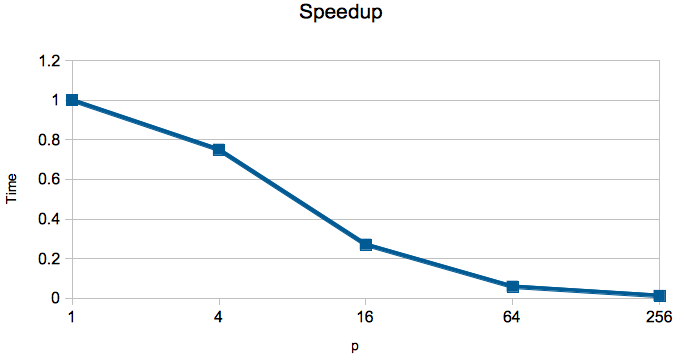
\includegraphics[width=.5\textwidth]{images/speedup.png}
   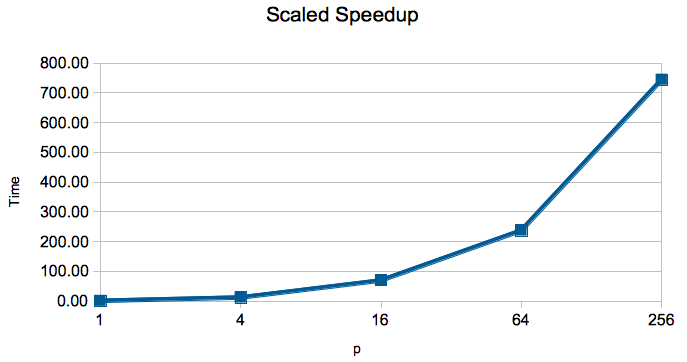
\includegraphics[width=.5\textwidth]{images/scaled_speedup.png}
 \end{figure}
 We can see from these figures that by using the scaled speedup
 shows a significantly larger speedup as $p$ is increased while
 the standard speedup reports a speedup of less than 1 as the
 number of processing elements is increased.\\
 
 {\bf 5.10 (Prefix sums)} Consider the problem of computing the
 prefix sums (Example 5.1) of $n$ numbers on $n$ processing
 elements. What is the parallel runtime, speedup, and
 efficiency of this algorithm? Assume that adding two numbers
 takes one unit of time and that communicating one number
 between two processing elements takes 10 units of time. Is the
 algorithm cost-optimal?\\\\
 The parallel runtime of this algorithm will be
 $(n/p-1)+11logp$. From here we can see the speedup is
 $\frac{n}{(n/p-1)+11logp}$ and the efficiency will be
 $\frac{n}{n-p+11plogp}$. This algorithm will be cost optimal so
 long as $n=\Omega(plogp)$.\\

 {\bf 5.13} The parallel runtime of a parallel implementation of
 the FFT algorithm with $p$ processing elements is given by $T_p =
 (n/p) log n + t_w(n/p) log p$ for an input sequence of
 length $n$ (Equation 13.4 with $t_s = 0$). The maximum number of
 processing elements that the algorithm can use for an $n$-point
 FFT is $n$. What are the values of $p_0$ (the value of $p$
 that satisfies Equation 5.21) and $T_P^{min}$ for $t_w = 10$?\\\\
 Equating the derivative with respect to $p$ of the right hand
 side of $T_p$ to zero we can solve for $p$ as follows:
 $$ \begin{array}{rclr}
   -\frac{nlogn}{p^2}+t_wn\frac{1-logp}{p^2} & = & 0\\
   -nlogn+t_wn(1-logp) & = & 0\\
   t_wn(1-logp) & = & nlogn\\
   t_w(1-logp) & = & logn\\
   1 - \frac{logn}{t_w} & = & logp\\
   logn & = & logp & \mbox{dropping 1 and $t_w$}\\
   n & = & p\\
 \end{array}
 $$
 This gives us a $p_0$ values of $n$. Substituting this into $T_p$
 we get and $t_w = 10$:
 $$ \begin{array}{rcl}
   T_p^{min} & = & \frac{nlogn}{n} + 10\frac{nlogn}{n}\\
   & = & logn + 10logn\\
   & = & 10logn\\
 \end{array}$$
\end{document}
